\chapter{Descripción del Experimento}
 
 Los detectores de propósito general en colisionadores de alta energía suelen tener capas de detección dispuestas en forma cilíndrica alrededor del eje del haz. Un ejemplo destacado de este tipo de detector es el Solenoide Compacto de Muones (CMS), una de las colaboraciones científicas internacionales más grandes de la historia y parte del LHC en el CERN. El CMS está diseñado para llevar a cabo una variedad de experimentos, incluidos los dedicados al estudio del Modelo Estándar. Este capítulo describe los componentes principales del detector CMS, con especial atención a los sistemas encargados de medir la luminosidad, enfocándose particularmente en el rastreador de píxeles de silicio, cuyo detalle es crucial para esta tesis.
 
\section{CMS (Compact Muon Solenoid)}

El experimento CMS es un detector de propósito general del LHC, compuesto por varias capas dedicadas a funciones específicas. El sistema central es un imán solenoide que genera un campo magnético de 4 teslas, el cual desvía partículas cargadas para medir su energía y momento. El detector tiene 21.6 metros de largo y 14.6 metros de diámetro, con un peso total de 14,000 toneladas \cite{CMS_Exp_2008}.\\

Las partículas cargadas deben ser desviadas al alejarse del punto de colisión, lo que se logra mediante un fuerte campo magnético. Este campo cumple dos funciones clave: primero, permite diferenciar las partículas cargadas positivamente de las negativamente cargadas, ya que se desplazan en direcciones opuestas bajo la influencia del mismo campo magnético; segundo, posibilita la medición del momento de la partícula.\\

Entre sus componentes, destaca el rastreador de silicio, que permite reconstruir trayectorias de partículas cargadas mediante píxeles y tiras de silicio. Este rastreador registra "hits" en las capas de detección, que luego se usan para calcular la trayectoria de las partículas.\\

\begin{center}
  \begin{figure}[ht]
    \centering
    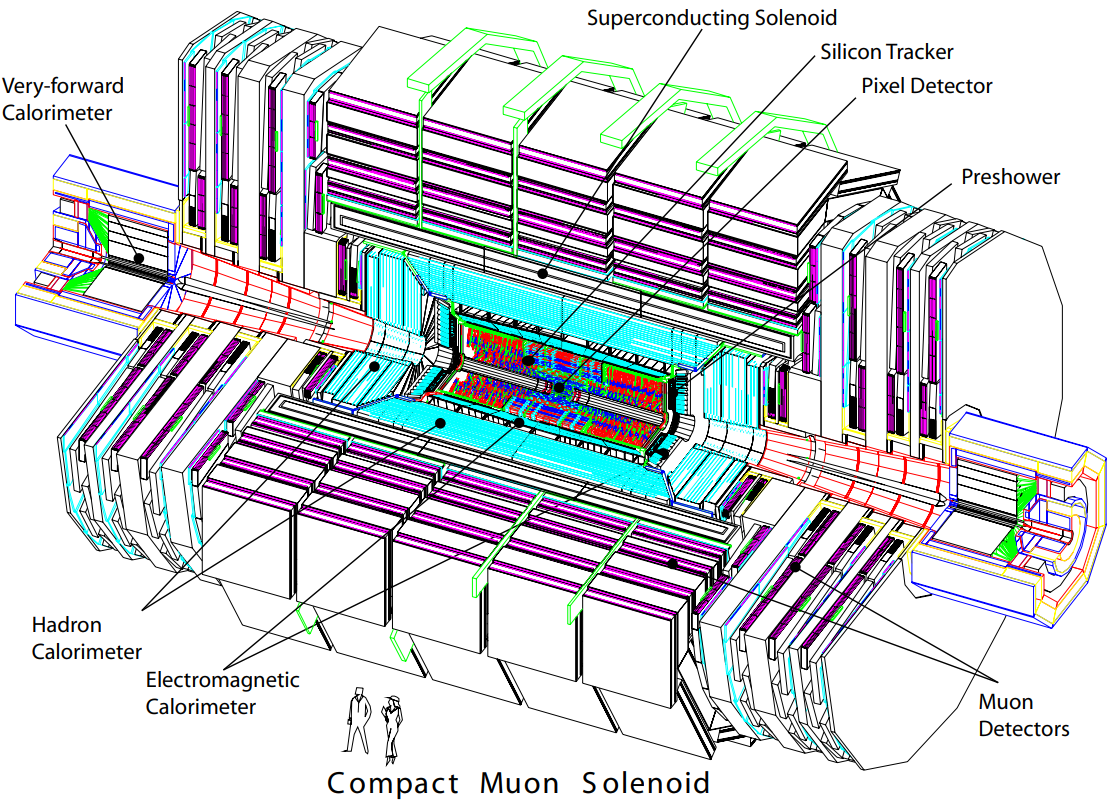
\includegraphics[scale=.3]{Chapter2/CMS_detector_simple.png}
    \caption[Vista panorámica del detector CMS]{Vista panorámica del detector CMS.}
    \label{detector_CMS}
  \end{figure}
\end{center}

El calorímetro electromagnético (ECAL) mide la energía de electrones y fotones a través de cristales de tungstato de plomo (PbWO4), mientras que el calorímetro hadrónico (HCAL) detecta hadrones y mide la energía de jets y la energía transversa perdida. Ambos calorímetros cubren diferentes secciones: el barril, los endcaps y el preshower para ECAL, y las secciones forward, endcap, barrel y outer para HCAL \cite{det_summary}.\\

Finalmente, el CMS cuenta con un sistema de detección de muones, que al ser más pesados que los electrones, atraviesan los calorímetros y son detectados en subdetectores ubicados dentro del yugo de acero del solenoide. Estos detectores permiten medir el momento de los muones dentro y fuera del campo magnético del CMS \cite{det_summary}.\\

\begin{center}
  \begin{figure}[ht]
    \centering
    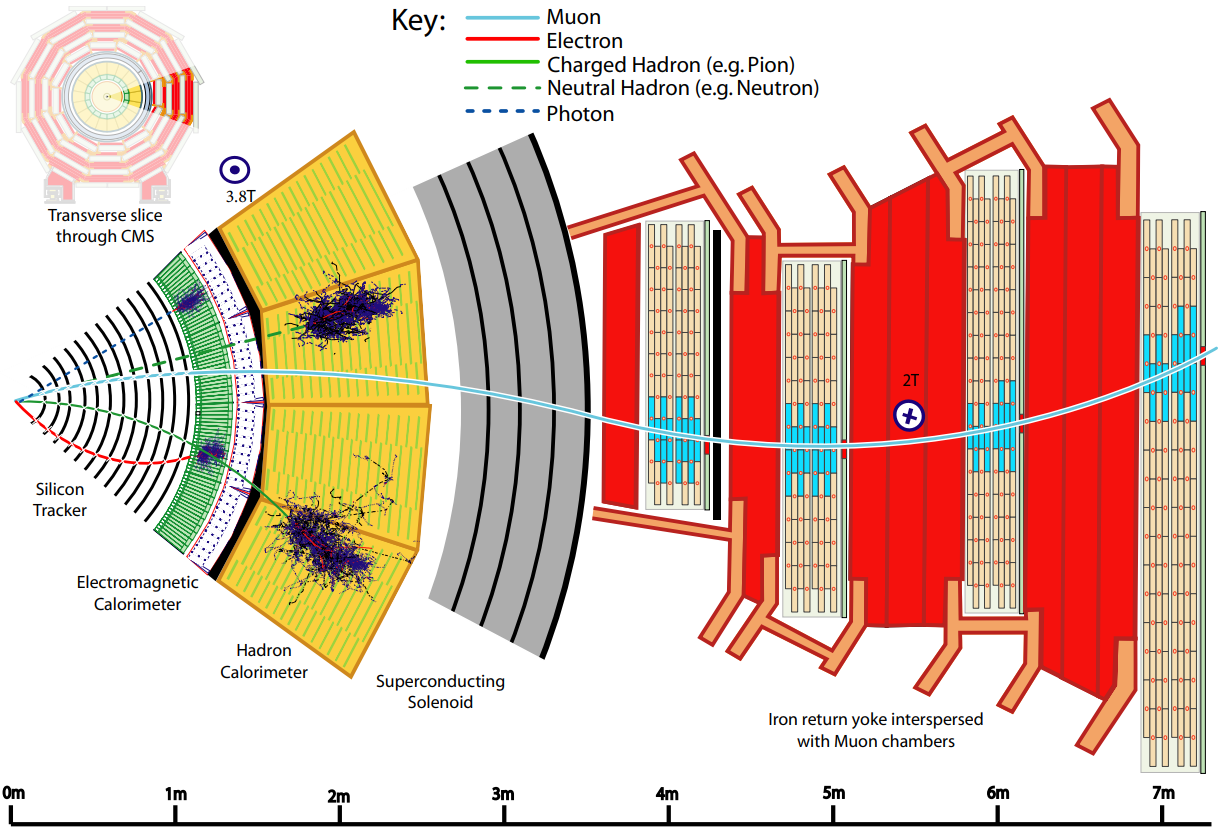
\includegraphics[scale=.3]{Chapter2/slice_det.png}
    \caption[Vista transversal del detector CMS.]{Vista transversal del detector CMS con algunas interacciones de partículas (desde la región de interacción del haz hasta el detector de muones).}
    \label{slice_CMS}
  \end{figure}
\end{center}

El sistema de coordenadas del CMS está centrado en el detector, con el eje $y$ orientado hacia arriba, el $x$ hacia el centro del LHC, y el $z$ alineado con el haz, permitiendo definir parámetros como el ángulo acimutal y la pseudorapidez \cite{det_summary}.\\

\section{Luminómetros en CMS}
\label{Luminometers}

El CMS utiliza siete sistemas para medir la luminosidad. Dos de ellos, el Pixel Luminosity Telescope (PLT) y el Fast Beam Condition Monitor (BCM1F), están diseñados específicamente para esta función, mientras que el calorímetro Hadronic Forward (HF) emplea un sistema de lectura dedicado. Además, existen tres métodos más: Drift Tube Luminosity (DT), el Pixel Cluster Counting Method (PCC) y el Vertex Counting Method (VTX), que utilizan datos del detector CMS y su sistema de adquisición de datos. Por último, los detectores RAMSES, destinados al monitoreo ambiental, también contribuyen a las mediciones de luminosidad \cite{pas_18}.\\

El PLT usa sensores de píxeles de silicio distribuidos en telescopios para medir coincidencias triples, lo que permite identificar trayectorias de partículas. En el HF, la medición se realiza con dos algoritmos: HFOC, basado en la ocupación de torres, y HFET, que usa la energía transversal. El método DT mide la tasa de "muon track stubs", pero no permite mediciones individuales por colisión. El BCM1F, con sensores de silicio y diamante, ofrece mediciones precisas y separa impactos de colisiones de los inducidos por la máquina. RAMSES, aunque no diseñado como luminómetro, puede medir la luminosidad detectando fotones. Finalmente, el PCC cuenta los clústeres de píxeles en el detector, proporcionando una medición adicional de luminosidad \cite{pas_18}.\\

La ubicación de los 7 luminómetros antes mencionados se muestran en la figura 2.3.\\

\begin{center}
  \begin{figure}[ht]
    \centering
    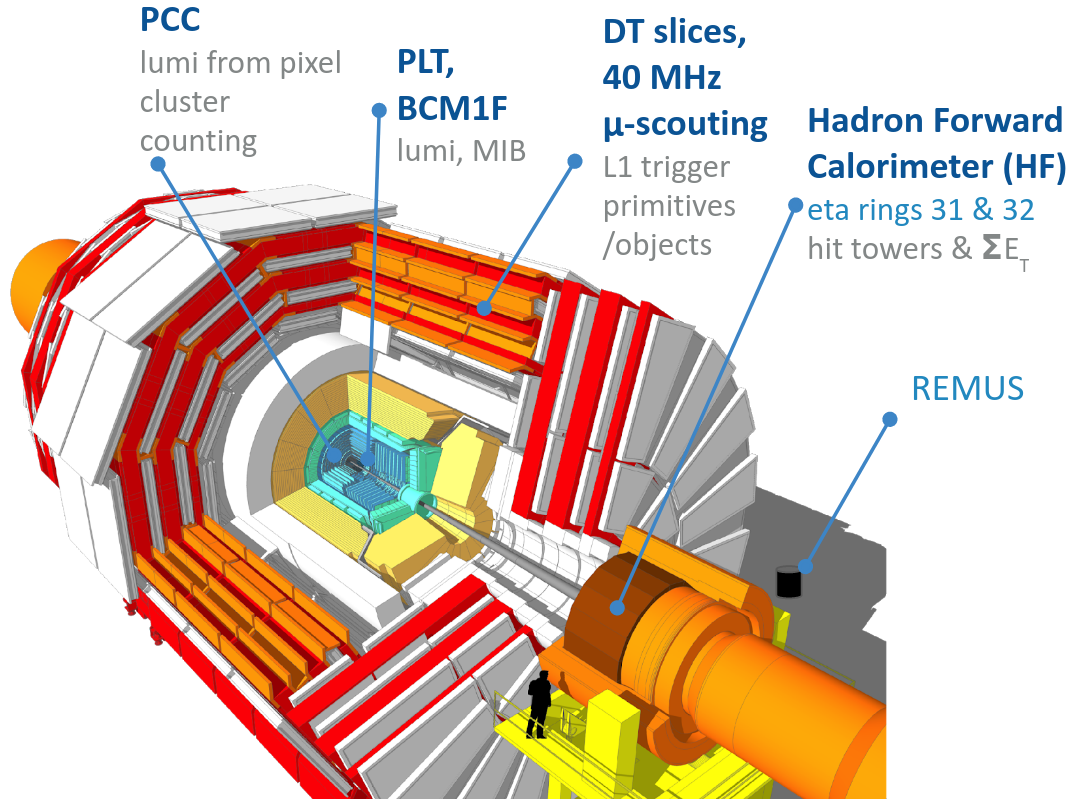
\includegraphics[scale=.3]{Chapter2/detectors.png}
    \caption[Luminómetros en CMS]{Los siete luminómetros que componen el sistema de medición de luminosidad de CMS son: BCM1F, HFET, HFOC, PLT, REMUS, DT y PCC.}
    \label{luminometers}
  \end{figure}
\end{center}

\section{Sistema de Rastreo del CMS}

El sistema de rastreo en el CMS es esencial para medir con precisión las trayectorias y momentos de las partículas cargadas y para reconstruir vértices secundarios. Este sistema tiene 5.8 metros de largo y 2.5 metros de diámetro, y está compuesto por dos subsistemas principales: el detector de píxeles y el rastreador de tiras (Strip tracker). El detector de píxeles se encuentra en el centro, rodeado por el rastreador de tiras, como se ilustra en la Figura 2.4 \cite{pas_18}.\\

El rastreador de tiras se divide en el Tracker Inner Barrel (TIB) y Tracker Inner Disks (TID), que tienen cuatro capas de barril y tres discos en cada endcap, y el Tracker Outer Barrel (TOB) junto con los Tracker EndCaps (TEC), que consisten en seis capas y nueve discos en los extremos. Este sistema cubre 198 $m^{2}$ con 15,148 módulos de silicio y alrededor de 9.3 millones de tiras, proporcionando una alta resolución en la medición de trayectorias.\\

El sistema permite medir la curvatura de las partículas en el campo magnético del solenoide, lo que facilita determinar su momento. Es crucial para identificar partículas como muones y electrones, y para reconstruir eventos complejos de colisiones de alta energía.\\

El rastreador de píxeles, la parte más interna, consta de cuatro capas concéntricas en el barril y tres discos en los endcaps. Con 124 millones de píxeles, permite una resolución extremadamente alta para medir las trayectorias de las partículas cercanas al punto de interacción. Su cobertura llega a una pseudorapidez de \( | \eta | < 2.5 \) y es clave para detectar partículas en eventos de alta densidad.\\

Los píxeles en cada capa se organizan en una matriz, permitiendo la medición de las coordenadas en dos dimensiones $(r, z)$, lo que contribuye a la reconstrucción precisa de las trayectorias de las partículas. En la siguiente sección, se detallarán más aspectos técnicos de este detector, incluyendo su funcionamiento y las características que lo hacen fundamental en la reconstrucción de eventos a alta precisión.\\


\begin{center}
  \begin{figure}[ht]
    \centering
    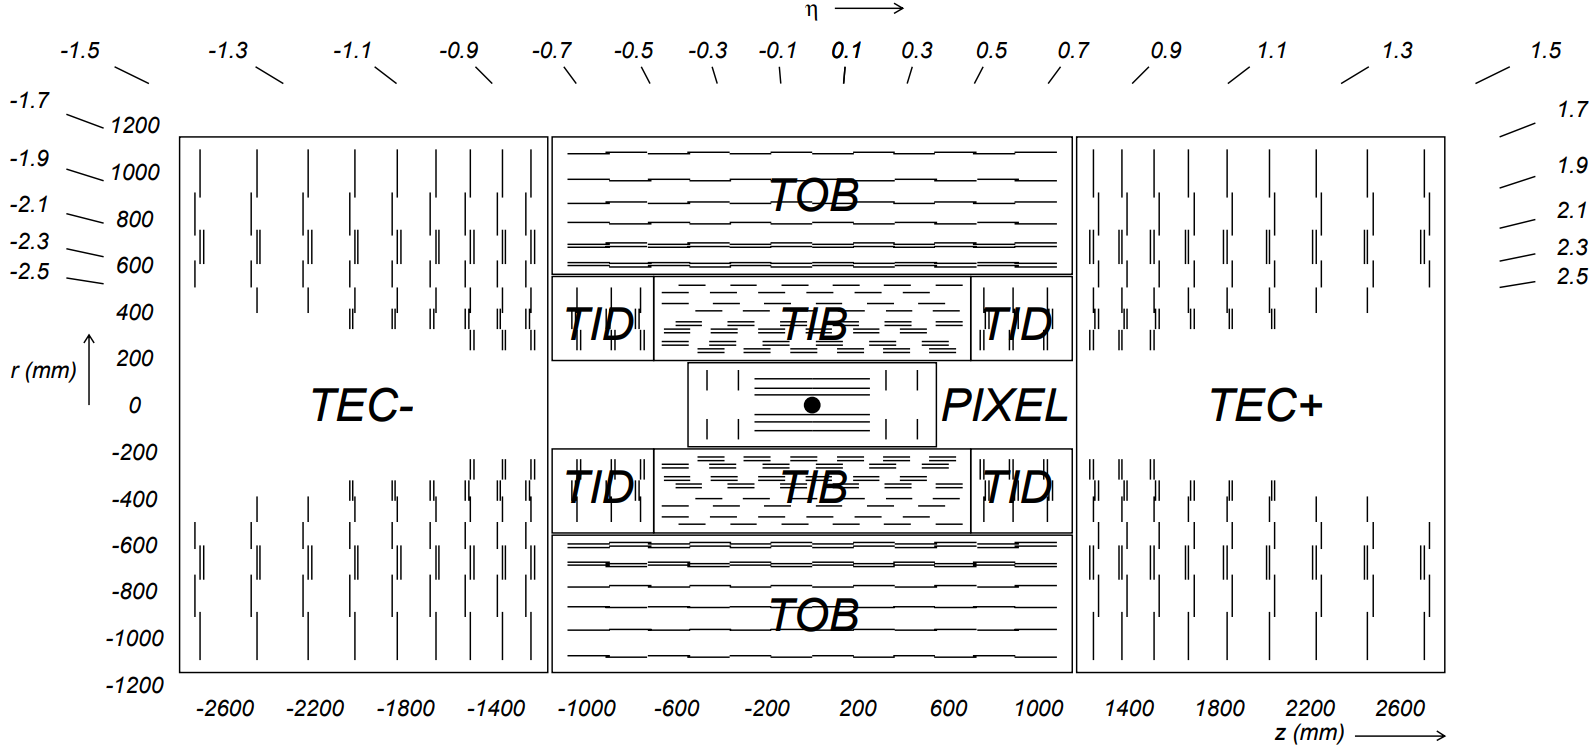
\includegraphics[scale=.23]{Chapter2/strip_layout.png}
    \caption[Corte transversal esquemático a través del rastreador del CMS.]{Corte transversal esquemático a través del rastreador del CMS.}
    \label{strip_layout}
  \end{figure}
\end{center}


\section{Silicon Pixel Detector}

El detector de píxeles de silicio forma el componente más interno del sistema de rastreo. Este detector proporciona una cobertura espacial completa en el área más cercana al punto de interacción, lo que permite un seguimiento preciso de las partículas cargadas y la reconstrucción de vértices. La cobertura del detector de píxeles se encuentra en el rango de pseudorapidez $(|\eta| < 2.5)$, operando en un entorno rico en radiación, caracterizado por una alta densidad de trayectorias \cite{phase1_Pixel_Detector}.\\

El detector de píxeles del CMS está compuesto por cuatro capas concéntricas en forma de barril (L1-L4), cada una con radios de 29, 68, 109 y 160 mm, y tres discos (D1-D3) en cada extremo, ubicados a distancias de 291, 396 y 516 mm del centro del detector. Todo el detector consta de 1856 módulos de sensores de silicio segmentados \cite{CMS_Exp_2008}.\\  

La Figura 2.5 muestra un esquema de la disposición del detector de píxeles de la Fase 1 del CMS, el cual cubre un área total de silicio de $1.9 m^{2}$. Los detectores BPIX y FPIX están equipados con cuatro medios cilindros de servicio cada uno, que tienen una longitud combinada de $540 mm$. Estos cilindros albergan los circuitos de lectura y control, además de proporcionar soporte para las líneas de alimentación y los tubos de refrigeración del detector \cite{phase1_Pixel_Detector}.\\

\begin{center}
  \begin{figure}[h]
    \centering
    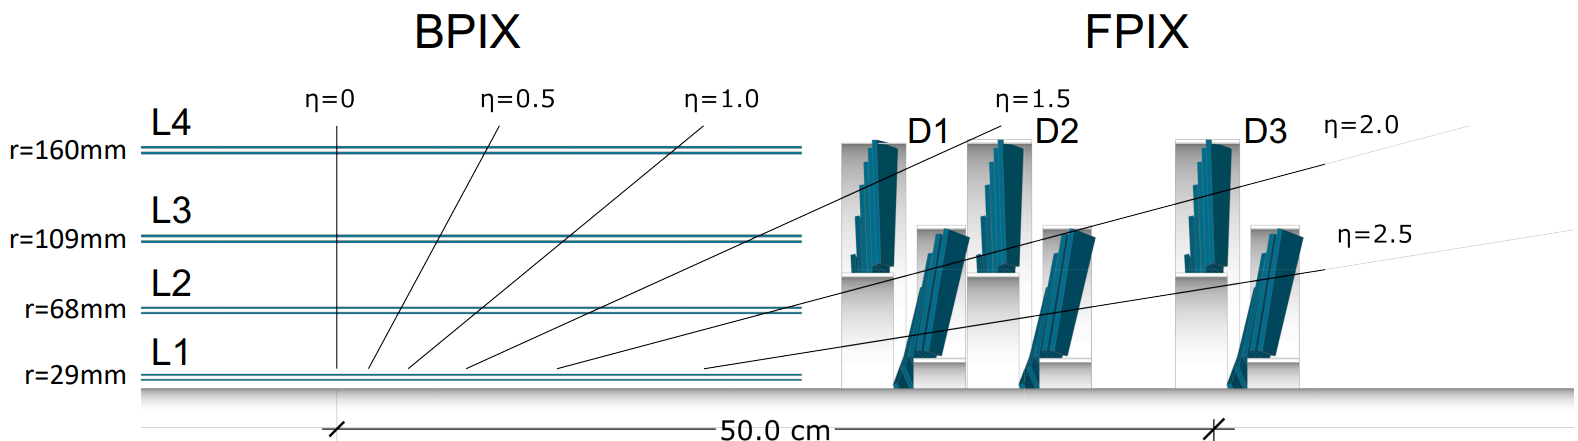
\includegraphics[scale=.26]{Chapter2/phase1_PixelDetector.png}
    \caption[Fase 1 del detector de pixeles en CMS]{Disposición del detector de píxeles de la Fase 1 del CMS en vista longitudinal.}
    \label{phase1_pixel_detector}
  \end{figure}
\end{center}

El detector BPIX está compuesto por dos mitades independientes, cada una de estas es autosuficiente desde el punto de vista mecánico. Cada mitad incluye un medio detector y dos semi-cilindros de servicio. Este detector consta de 1184 módulos de sensores de silicio segmentados, y la orientación de las superficies de cada módulo es paralela al campo magnético en ambas mitades.\\

A diferencia del BPIX, el detector FPIX está dividido en cuatro cuadrantes, que operan de manera independiente entre sí. Cada cuadrante incluye tres medio-discos que se alojan dentro de un semi-cilindro de servicio. La disposición de los sensores se ajusta de modo que el lado más largo de los píxeles esté alineado radialmente. El detector FPIX está compuesto por un total de 672 módulos de sensores de silicio segmentados, que se distribuyen entre anillos internos y externos, con 22 y 34 módulos respectivamente.\\

Un módulo del detector de píxeles está formado por un sensor de silicio plano con dimensiones de 18.6 $\times$ 66.6 $mm^{2}$, que abarca un área activa de 116.2 $\times$ 64.8 $mm^{2}$. Este sensor está compuesto por 160 $\times$ 416 píxeles, que están conectados a una matriz de 2 por 8 chips de lectura (ROC) mediante una soldadura de bump. Cada chip de lectura contiene 4160 canales, encargados de medir la altura del pulso de cada píxel. En total, el detector cuenta con 124 millones de canales de lectura. El tamaño estándar de cada píxel es de 100 $\times$ 150 $\mu m^{2}$.\\

\begin{center}
  \begin{figure}[h]
    \centering
    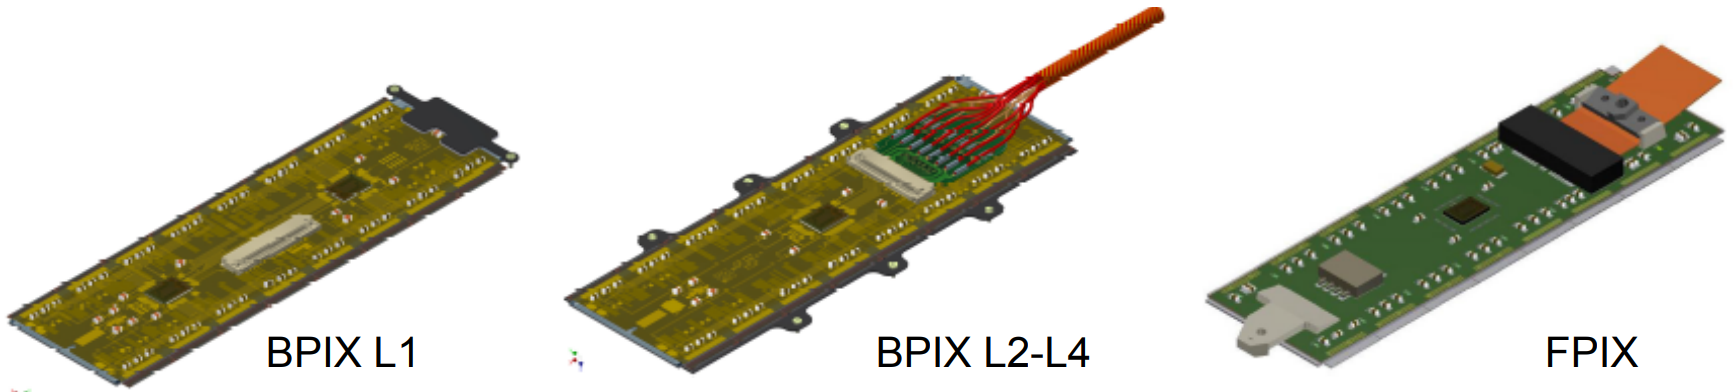
\includegraphics[scale=.2]{Chapter2/modules_drawing.png}
    \caption[Tipos de módulos en el detector de pixeles]{Estas son ilustraciones de los módulos del detector de píxeles utilizados en los detectores BPIX L1 (izquierda), BPIX L2-L4 (centro) y FPIX (derecha).}
    \label{modules_drawing}
  \end{figure}
\end{center}

La Figura 2.6 ilustra los módulos del detector de píxeles de la Fase-1 del CMS, mientras que la Figura 2.7, a la izquierda, muestra el diseño del sensor de silicio conectado al chip de lectura. En el lado derecho de la Figura 2.7, se puede ver una partícula cargada atravesando un píxel, proporcionando suficiente energía para expulsar electrones de los átomos de silicio. Un voltaje aplicado al sensor permite la recolección de estas cargas como una pequeña señal eléctrica, que luego es amplificada por un chip electrónico de lectura \cite{phase1_Pixel_Detector}.\\

\begin{center}
  \begin{figure}[h]
    \centering
    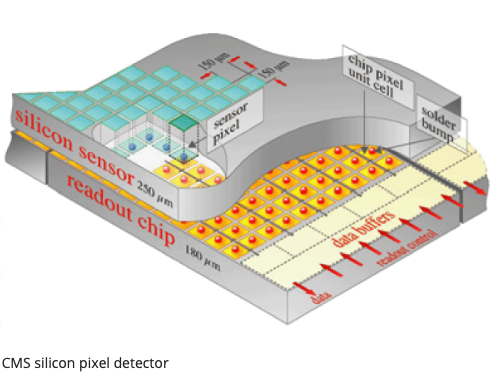
\includegraphics[scale=.3]{Chapter2/PixelSensor.png} 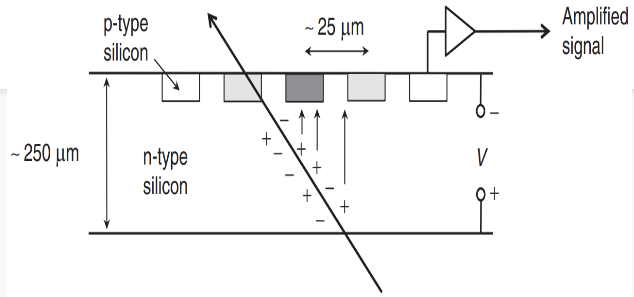
\includegraphics[scale=.3]{Chapter2/hit.png}
    \caption[Vista esquemática de un sensor de píxeles y su conexión a los canales de lectura]{Izquierda: diseño del sensor de píxeles conectado a un chip de lectura. Derecha: detección de impactos en un píxel correspondiente del sensor.}
    \label{module and hit}
  \end{figure}
\end{center}

\section{Reconstrucción del Pixel Cluster}

El proceso de reconstrucción de trayectorias involucra varios pasos. Primero, se identifican las señales que superan un umbral específico en los canales de píxeles y se utilizan para crear clústeres. Cada clúster representa la carga depositada por una sola partícula cargada. Posteriormente, se estiman la posición y las incertidumbres de los clústeres en un sistema de coordenadas local y ortogonal con respecto al plano del sensor \cite{Track_Reco_2014}.\\

Para que un clúster sea considerado válido, debe tener una carga de al menos 4000 electrones \cite{Track_Reco_2014,phase1_Pixel_Detector}. Las partículas mínimamente ionizantes (MIP) que atraviesan un sensor de silicio con un grosor de 285 $\mu m$ suelen depositar una energía equivalente a unos 21,000 electrones cuando inciden normalmente. Sin embargo, esta carga generalmente se dispersa en más de un píxel debido a la deriva de Lorentz, que provoca que los electrones sean desplazados por la fuerza generada por el campo electromagnético, lo que lleva a la formación de clústeres de carga.\\

La Figura 2.8 muestra un ejemplo de cómo se construye un clúster de píxeles. Cada cuadro en la figura representa un píxel. Los píxeles rojos indican que tienen la carga requerida, de hasta 2000 electrones, para ser considerados píxeles válidos y, por lo tanto, se incluyen en el clúster. Por otro lado, los píxeles verdes corresponden a depósitos de carga por debajo del umbral de 2000 electrones y no se incluyen en el clúster. La línea azul punteada en la figura representa la trayectoria de la partícula que viaja paralela al plano $xz$. A medida que avanza, activa píxeles en su camino de manera precisa, así como píxeles que se desvían de su trayectoria debido a la deriva de Lorentz \cite{Pixel_Hit_Reconstruction}.

\begin{center}
  \begin{figure}[h]
    \centering
    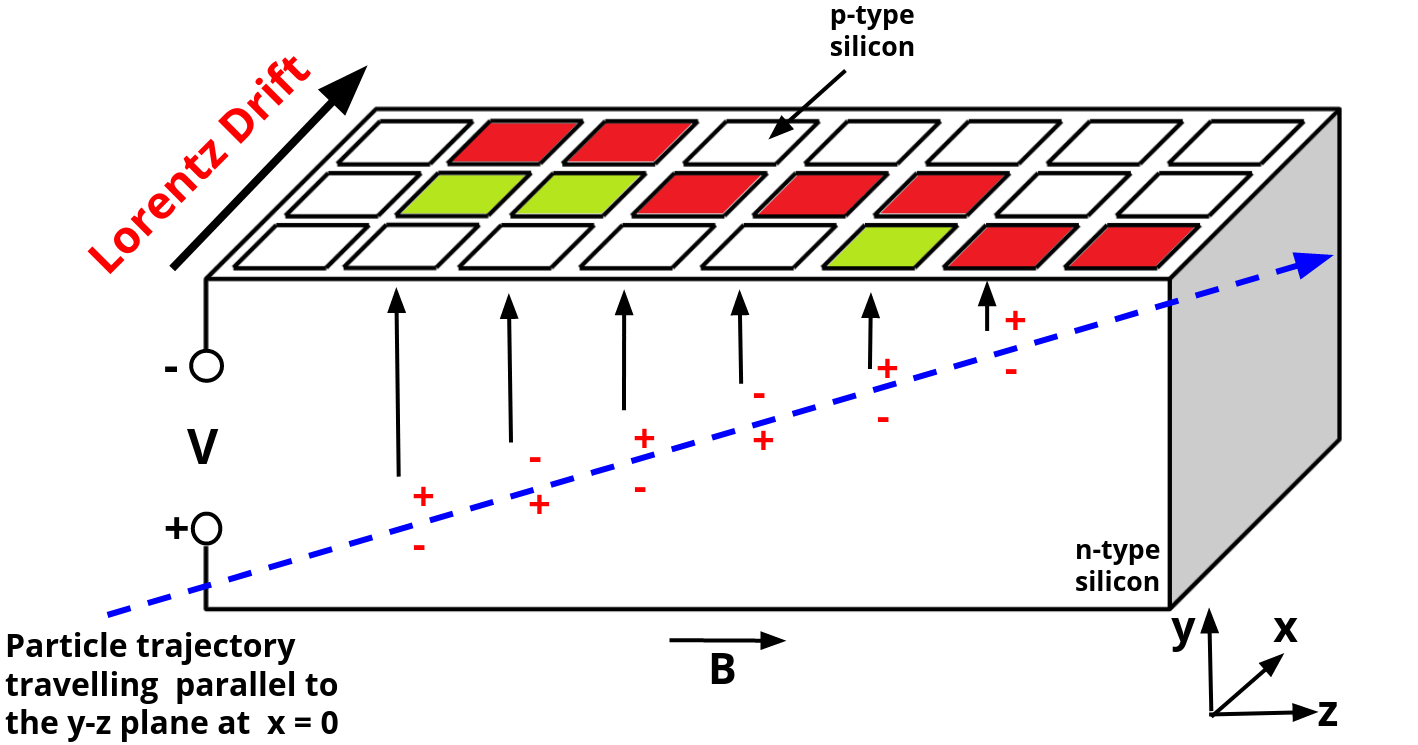
\includegraphics[scale=.25]{Chapter2/pixel_cluster.png} 
    \caption[Construcción de un pixel cluster]{La figura ilustra un ejemplo de un clúster de píxeles con una carga total de 4,000 electrones, que es el umbral necesario para que el clúster sea válido. Los píxeles rojos tienen la carga requerida, mientras que el píxel verde no alcanza el umbral.}
    \label{cluster}
  \end{figure}
\end{center}
